\ylDisplay{Dioodid} % Ülesande nimi
{Jaan Kalda} % Autor
{lahtine} % Voor
{2012} % Aasta
{G 8} % Ülesanne nr.
{8} % Raskustase
{
% Teema: Elektriahelad
\ifStatement
\begin{wrapfigure}{r}{0.4\linewidth}
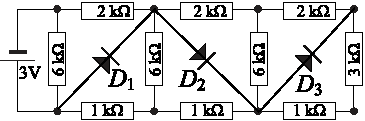
\includegraphics[width=\linewidth]{2012-lahg-08-dioodid}
\end{wrapfigure}
Millised võimsused eralduvad skeemil märgitud dioodidel? Dioodide voolu võib lugeda
nulliks kõikide vastupingete jaoks ning samuti ühest voldist
väiksemate päripingete jaoks; suvalise pärivoolu puhul on dioodi pinge
\SI{1,0}V. Takistite takistused ja elektromotoorjõu väärtus on toodud
joonisel. Dioodi skeemitähise noole suund näitab pärivoolu
suunda.
\fi


\ifHint
Oluline on tähele panna, et dioodidel saab pärivoolu korral pingeks olla ainult \SI{1,0}{V}. Tasub vaadata, kas rohkem kui ühel dioodil saab üldse vastava skeemi korral selline pinge olla.
\fi


\ifSolution
Esimesele dioodile ($D_1$) ei saa langeda üle ühe voldi, mistõttu järgnevatele ($D_2$ ja $D_3$) peab langema alla ühe voldi (takisti võtab ka endale teatud pinge).
Seetõttu on ülejäänud dioodid suletud, st nullvooluga ning need võib skeemilt "välja lõigata". Selle tulemusel moodustub esimese dioodi taha 
jada- ja rööpühenduste kombinatsioon kogutakistusega $\SI 4{k\ohm}$, millele langeb dioodipinge 1V ning mida läbib vool $\SI 1V /\SI 4{k\ohm}= \SI {0,25}{mA}$. 
Esimesele kahe kilo-oomisele takistile langeb pinge $\SI 3V-\SI 1V=\SI 2V$, mistõttu selle vool on $\SI 2V/\SI 2{k\ohm}=\SI 1{mA}$. Järelikult on esimese dioodi vool
$\SI 1{mA}-\SI {0,25}{mA}=\SI{0,75}{mA}$ ning võimsus $\SI{0,75}{mA}\cdot \SI 1V=\SI{0,75}{mW}$. Suletud dioodidel võimsust loomulikult ei eraldu.
\fi


\ifEngStatement
% Problem name: Diodes
\begin{wrapfigure}{r}{0.4\linewidth}
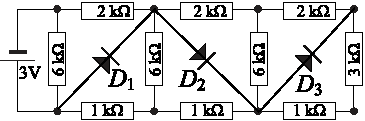
\includegraphics[width=\linewidth]{2012-lahg-08-dioodid}
\end{wrapfigure}
What powers are dissipated by the diodes marked in the figure’s circuit? Assume that the current of the diodes is zero for all the reverse voltages and also for forward voltages below one volt. For a random forward voltage the voltage of the diode is 1,0 V. The values of resistors’ resistances and the electromotive force are marked in the drawing. The direction of a diode’s arrow in the drawing shows the direction of the forward voltage.
\fi


\ifEngHint
It is important to notice that the voltage of the diodes for forward current can only be 1.0 V. You should see if more than one diode can even have such a voltage for the corresponding scheme.
\fi


\ifEngSolution
The voltage applied to the first diode ($D_1$) cannot be over one volt which is why the next diodes ($D_2$ and $D_3$) must be applied with a voltage below one volt (the resistor takes a certain voltage on it as well). This is why the rest of the diodes are closed meaning that they have zero current and they can be “cut out” of the diagram. This results in a combination of series and parallel connections behind the diode that has the total resistance $\SI 4{k\ohm}$. The diode’s voltage 1V is applied to the combination and the current $\SI 1V /\SI 4{k\ohm}= \SI {0,25}{mA}$ goes through it. The voltage $\SI 3V-\SI 1V=\SI 2V$ is applied to the first 2 ohm resistor which is why its current is $\SI 2V/\SI 2{k\ohm}=\SI 1{mA}$. Therefore the current of the first diode is $\SI 1{mA}-\SI {0,25}{mA}=\SI{0,75}{mA}$ and the power $\SI{0,75}{mA}\cdot \SI 1V=\SI{0,75}{mW}$. Naturally no power is dissipated by the closed diodes.
\fi
}